\documentclass[a4paper,12pt]{article}
\usepackage[T2A]{fontenc}
\usepackage[utf8]{inputenc}
\usepackage[english,russian]{babel}
\usepackage{listings}

\usepackage{amsmath}
\usepackage{MnSymbol}
\usepackage{wasysym}
\usepackage{indentfirst}

\usepackage{pgfplots}
\pgfplotsset{compat=1.9}

\usepackage{geometry}
\geometry{left=2cm}
\geometry{right=1.5cm}
\geometry{top=1cm}
\geometry{bottom=2cm}

\usepackage{graphicx}
\graphicspath{{img/}}
\DeclareGraphicsExtensions{.pdf,.png,.jpg}

\newcommand{\anonsection}[1]{\section*{#1}\addcontentsline{toc}{section}{#1}}

\lstset{
    language=C++,
    numbers=left,
    frame=single,
    texcl=true
}

\begin{document}

\begin{titlepage}

    \begin{center}
        \large
        Государственное образовательное учреждение высшего профессионального образования\\
        “Московский государственный технический университет имени Н.Э.Баумана”
        \vspace{3cm}

        \textsc{Дисциплина: Анализ алгоритмов}
        \vspace{0.5cm}

        \textsc{Лабораторная работа №1}
        \vspace{3cm}

        {\LARGE РЕДАКЦИОННОЕ РАССТОЯНИЕ}
        \vspace{3cm}

        Студент группы ИУ7-53,\\
        Степанов Александр Олегович
        \vfill
    \end{center}

    \begin{flushright}
        \begin{tabular}{l}
            Преподаватели:\\
            Строганов Юрий Владимирович\\
            Волкова Лилия Леонидовна
        \end{tabular}
    \end{flushright}

    \begin{center}

        2019 г.

    \end{center}

\end{titlepage}

\tableofcontents

\newpage
\anonsection{Введение}

В данной лабораторной работе ставятся следующие задачи:

\begin{enumerate}
    \item Изучение алгоритмов Левенштейна и Дамерау-Левенштейна нахождения
        расстояния между строками
    \item Получение практических навыков реализации указанных алгоритмов:
        двух алгоритмов в матричной версии и оного из алгоритмов в рекурсивной
        версии
    \item Сравнительный анализ линейной и рекурсивной реализации выбранного
        алгоритма определения расстояния между строками по затрачиваемым
        ресурсам (времени и памяти)
    \item Экспериментальное подтверждение различий во временой эффективности
        рекурсивной и нерекурсивной реализации выбранного алгоритма
        определения расстояния межлу строками при помощи разработанного
        программного обеспечения на материале замеров процессорного времен
        выполнения реализации на варьирующихся длинах строк
\end{enumerate}

\newpage
\section{Аналитическая часть}

\subsection{Описание задачи}

\textbf{Редакционное расстояние (расстояние Левенштейна)}
между двух строк - это
минимальное количество операций вставки одного символа, удаления одного
символа или замены одного символа на другой необходимых для превращения
одной строки в другую.

Для двух строк $S_1$ и $S_2$ с длинами $n$ и $m$ соотвественно можно
построить матрицу $D(n+1, m+1)$, в которой каждый элемент равен

\begin{equation}
D(i,j) =
\begin{cases}
    0, \text{ если } i = 0, j = 0 \\
    i, \text{ если } j = 0 \\
    j, \text{ если } i = 0 \\
    \min
    \left(
        \begin{matrix}
            D(i, j - 1) + 1 \\
            D(i - 1, j) + 1 \\
            D(i - 1, j - 1) +
            \begin{cases}
                0, \text{ если } S_1[i] \ne S_2[j] \\
                0, \text{ иначе}
            \end{cases}
        \end{matrix}
    \right)
    , \text{ иначе}
\end{cases}
\end{equation}

После нахождения каждого элемента матрицы, редакционное расстояние между
$S_1$ и $S_2$ будет в нижнем правом элементе матрицы.

\textbf{Расстояние Дамерау-Левенштейна} - это редакционное расстояние,
к которому добавляется еще одно действие - транспозиция (смена местами
двух соседних символов). Необходимо это потому, что около 80\% ошибок
при наборе текста человеком является транспозиция, как показал Дамерау.

По аналогии с расстоянием Левенштейна, здесь тоже используется матрица
$D(n+1, m+1)$ для строк $S_1$ и $S_2$ с длинами $n$ и $m$

\begin{equation}
D(i,j) =
\begin{cases}
    0, \text{ если } i = 0, j = 0 \\
    i, \text{ если } j = 0 \\
    j, \text{ если } i = 0 \\

    \min
    \left(
        \begin{matrix}
            D(i, j - 1) + 1 \\
            D(i - 1, j) + 1 \\
            D(i - 1, j - 1) +
            \begin{cases}
                0, \text{ если } S_1[i] \ne S_2[j] \\
                0, \text{ иначе}
            \end{cases} \\
            D(i - 2, j - 2) + 1
        \end{matrix}
    \right) \\
    , \text{ если } i > 1, j > 1, S_1[i] = S_2[j - 1], S_2[j] = S_1[i - 1] \\

    \min
    \left(
    \begin{matrix}
        D(i, j - 1) + 1 \\
        D(i - 1, j) + 1 \\
        D(i - 1, j - 1) +
        \begin{cases}
            0, \text{ если } S_1[i] \ne S_2[j] \\
            0, \text{ иначе}
        \end{cases}
    \end{matrix}
    \right)
    , \text{ иначе}
\end{cases}
\end{equation}

Расстояние Левенштейна и Дамерау-Левенштейна активно применяется:

\begin{itemize}
    \item для исправления ошибок в слове (в поисковых системах, базах
        данных, при вводе текста, при автоматическом распознавании
        отсканированного текста или речи).

    \item для сравнения текстовых файлов утилитой diff и ей подобными.

    \item в биоинформатике для сравнения генов, хромосом и белков.
\end{itemize}

\subsection{Пути решения}

Впервые эту задачу поставил советский математик Владимир Левенштейн при
изучении последовательностей 0-1.

Недавно Фредерих Дамерау доказал, что пользователи совершают очень много
ошибок транспозиции при наборе текста, поэтому расстояние
Дамерау-Левенштейна дает более лучшие результаты, чем обычное редакционное
расстояние.

\subsection{Выводы}

Редакционное расстояние широко применяется в областях программирования и
биоинформатики. Для алгоритмов Левенштейна и Дамерау-Левенштейна
используются операции вставки символа, удаления символа, замены символа и
транспозиции двух соседних символов. В данной работе будет проведено
исследование и сравнение этих алгоритмов.

\newpage
\section{Конструкторская часть}

В данной работе для нахождения расстояния Левенштейна используется матричный
алгоритм, а для Дамерау-Левенштейна матричнй и рекурсивный. Далее будут
рассмотрены все эти алгоритмы.

\subsection{IDEF0}

\begin{center}
    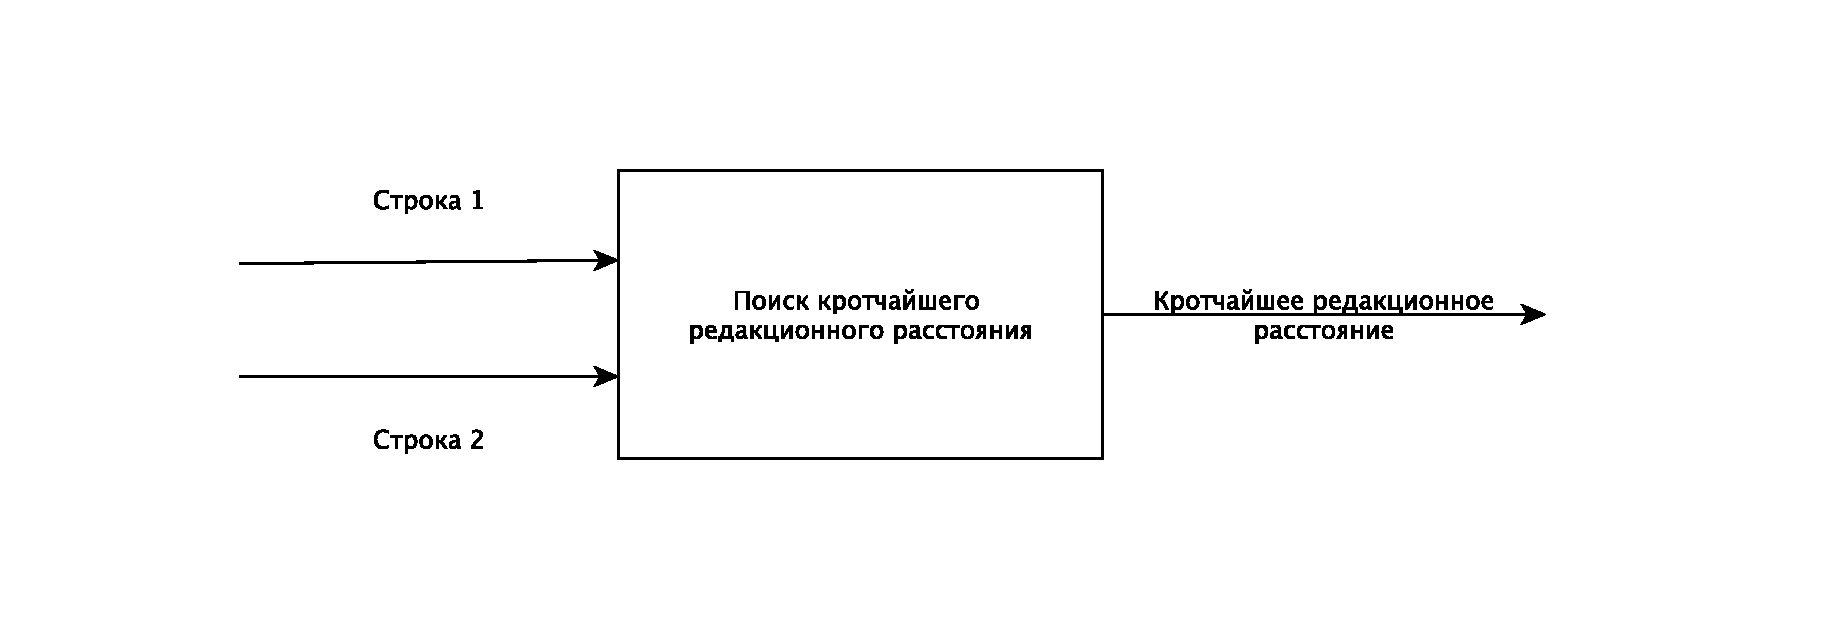
\includegraphics[scale=0.5]{IDEF0}
\end{center}

\subsection{Схемы алгоритмов}

\subsubsection{Матричный алгоритм Левенштейна}

\begin{center}
    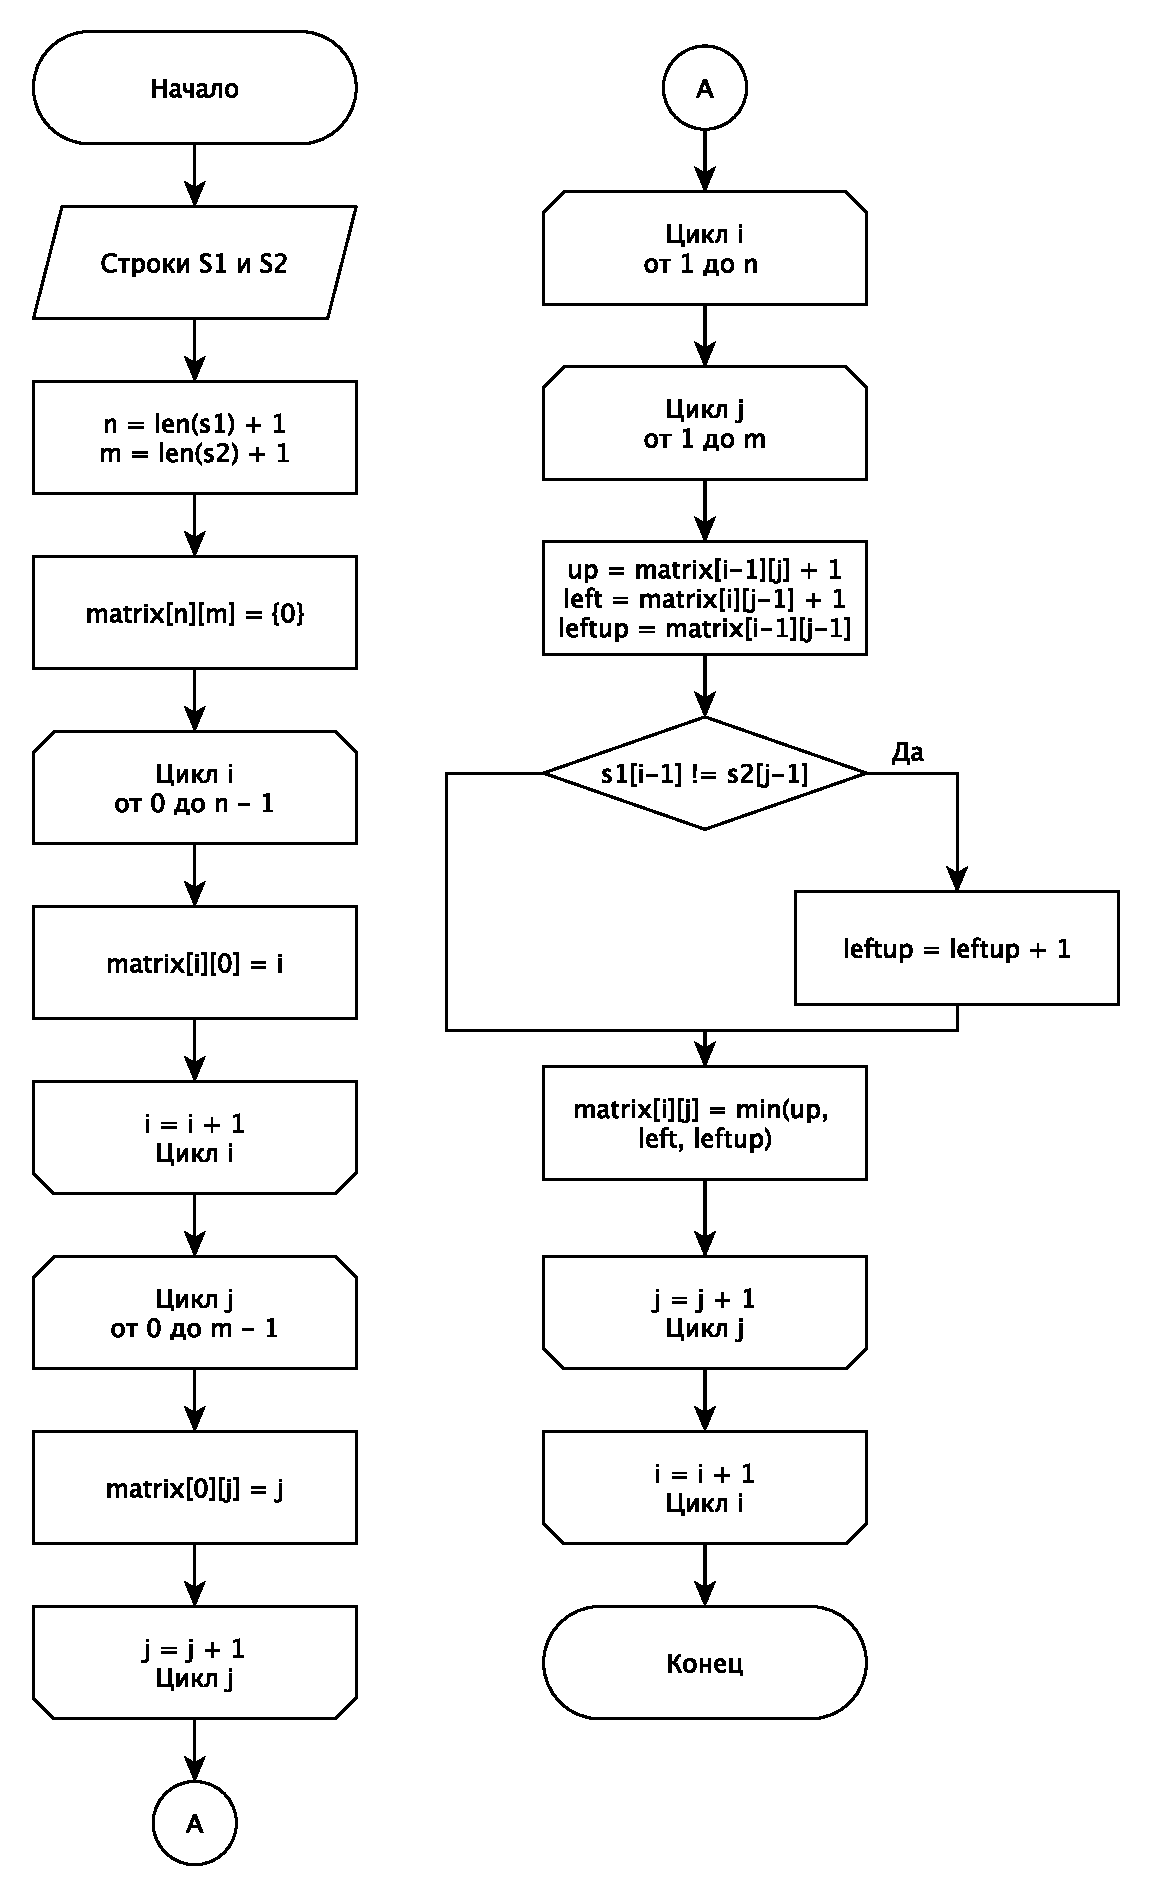
\includegraphics[scale=0.23]{Lmatrix}

    Схема 1. Матричный алгоритм Левенштейна
\end{center}

\subsubsection{Матричный алгоритм Дамерау-Левенштейна}

\begin{center}
    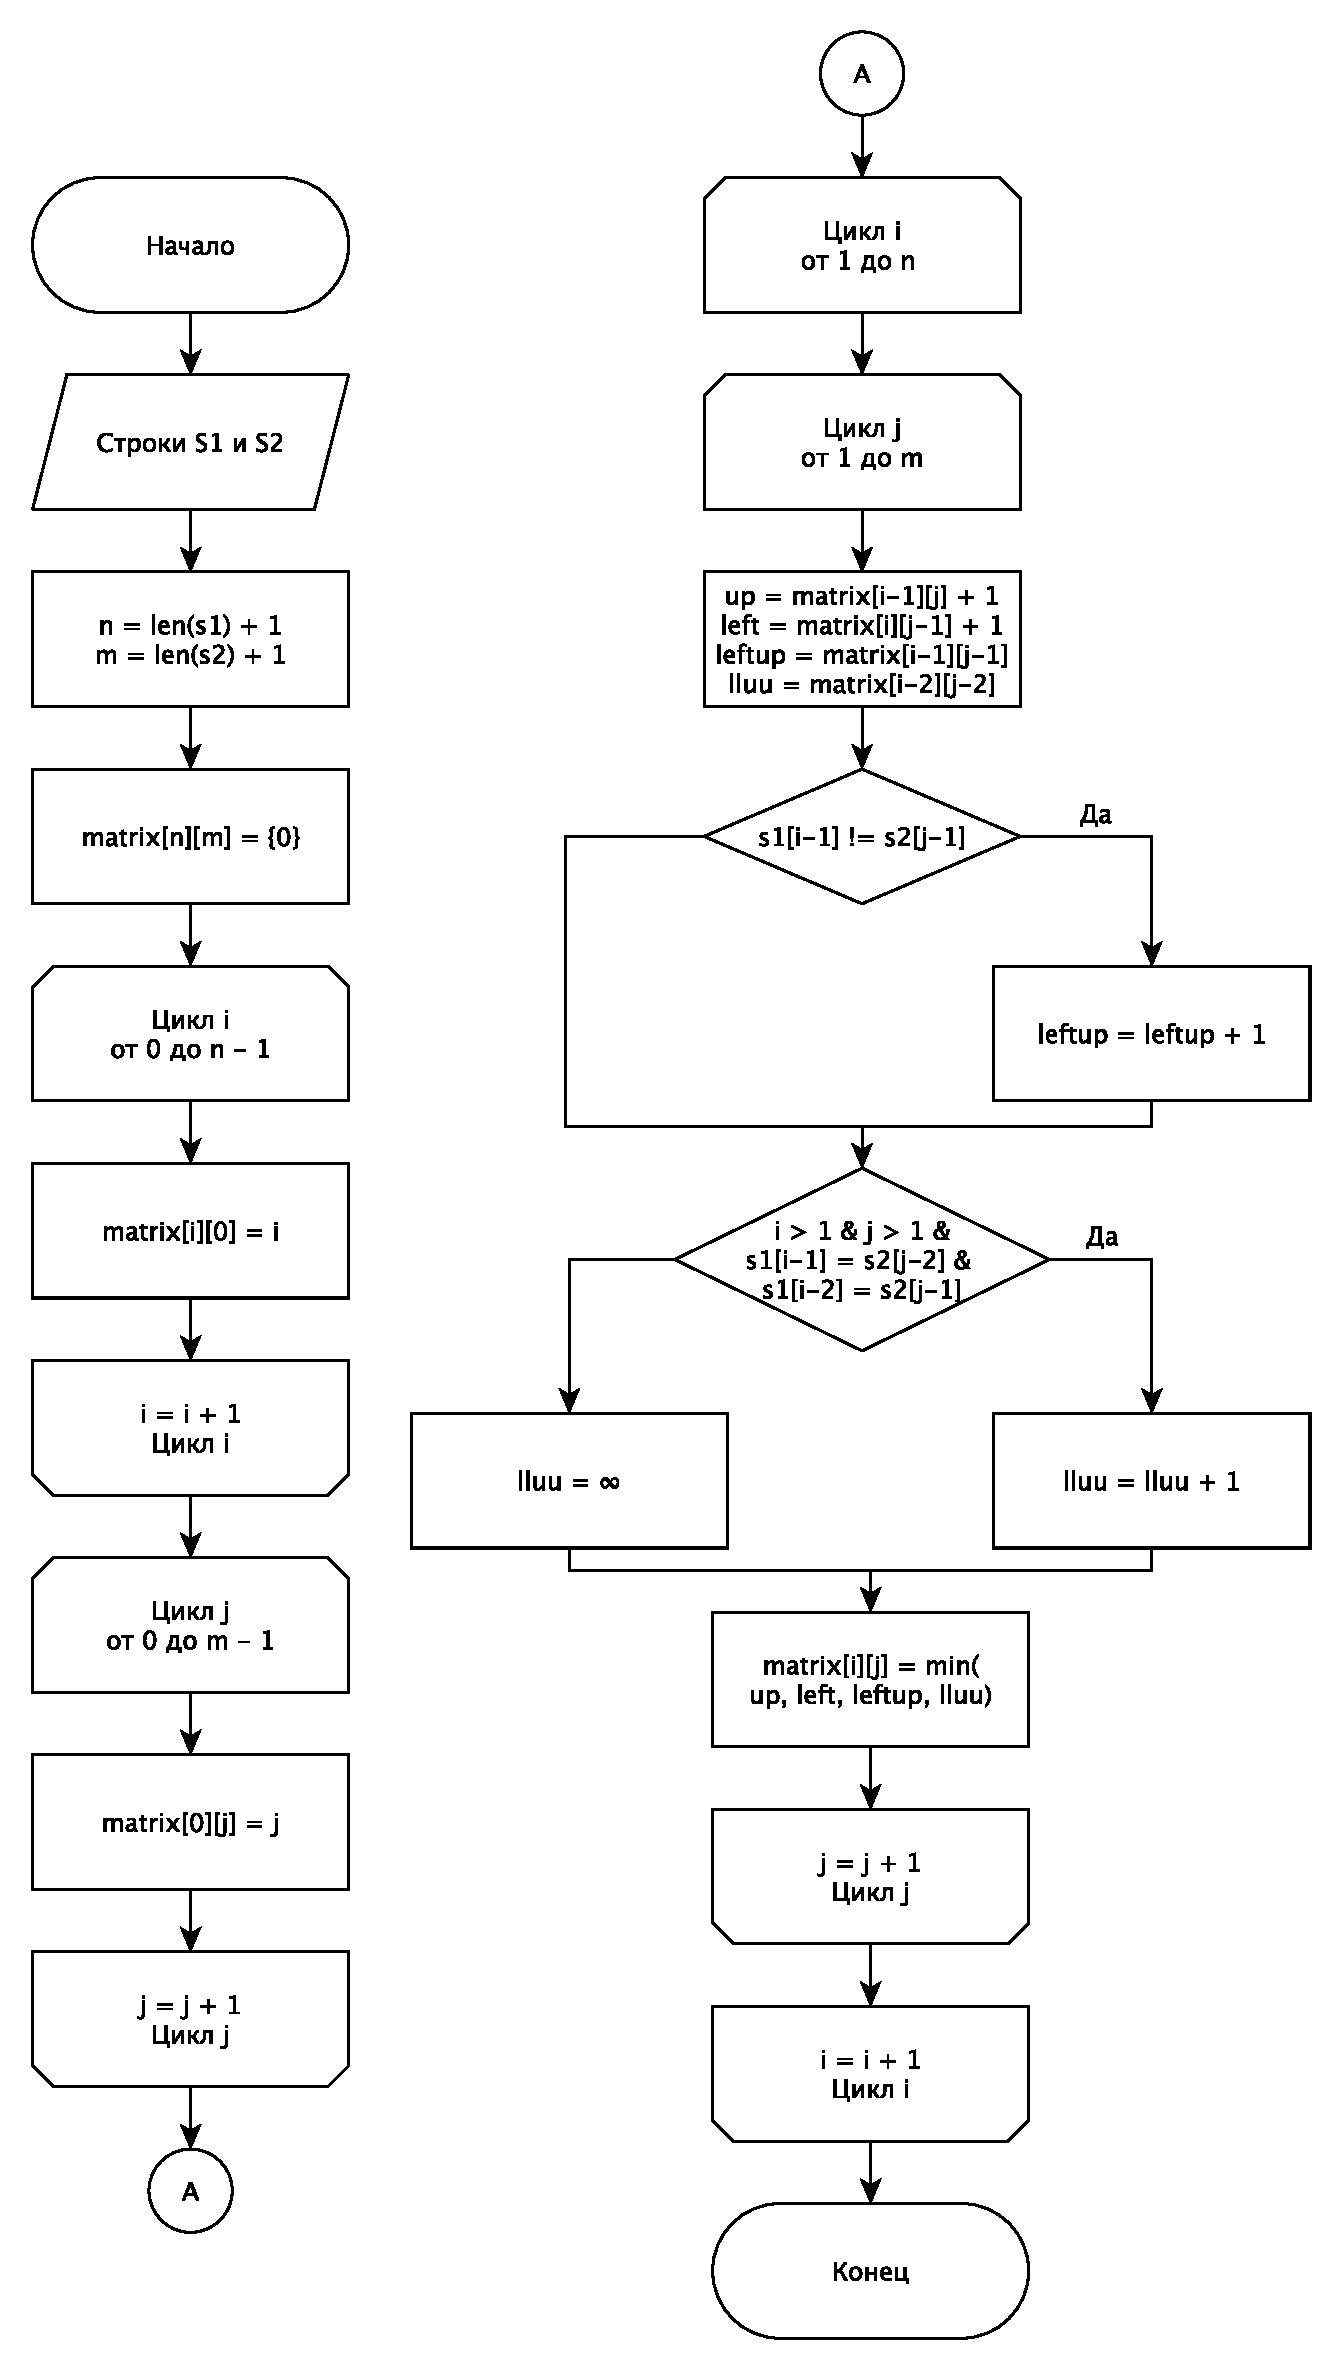
\includegraphics[scale=0.35]{DLmatrix}

    Схема 2. Матричный алгоритм Дамерау-Левенштейна
\end{center}

\subsubsection{Рекурсивный алгоритм Дамерау-Левенштейна}

\begin{center}
    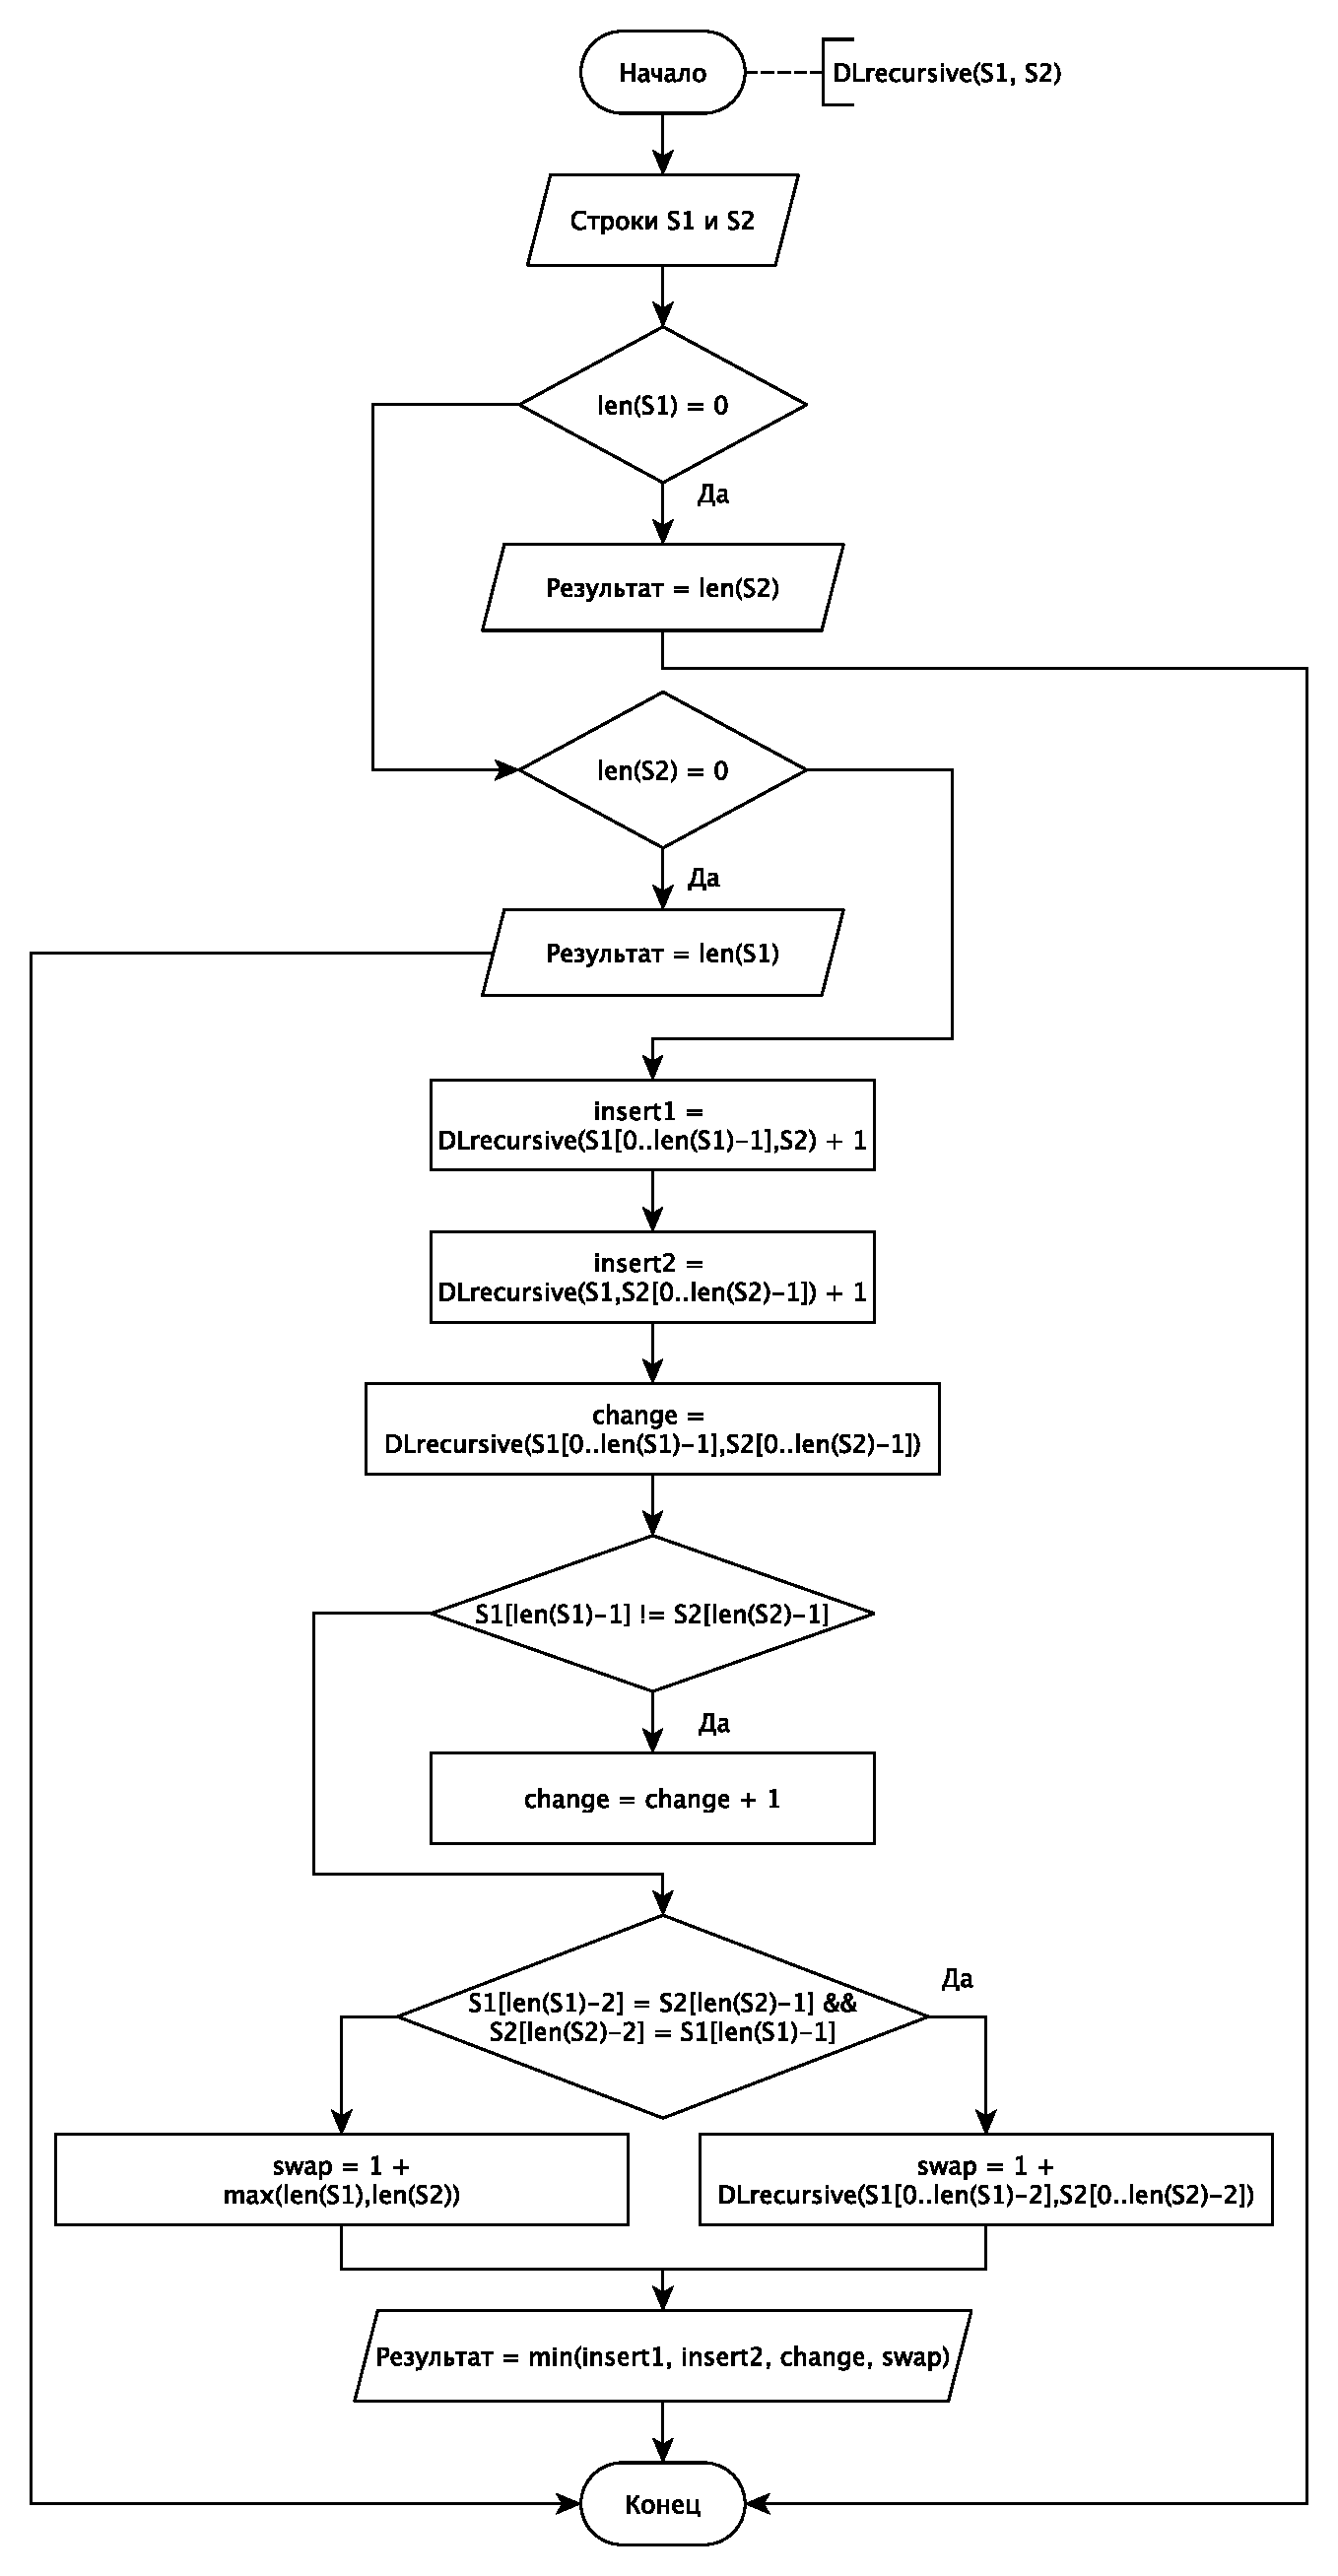
\includegraphics[scale=0.5]{DLrecursive}

    Схема 3. Рекурсивный алгоритм Дамерау-Левенштейна
\end{center}

\subsection{Выводы}

Рекурсивный алгоритм имеет сложность $\Omega (4^{max(n,m)})$, а матричные
$\Omega (n \cdot m)$. Таким образом очевидвидно, что рекурсивный алгоритм
сильно проигрывает матричным по времени. Проверим данное предположение
на реализованных алгоритмах.

\newpage
\section{Технологическая часть}

\subsection{Требования к программному обеспечению}

Программное обеспечение должно обеспечивать замер процессорного времени
выполнения каждого алгоритма. Проводятся замеры для случайно генерируемых
строк размерности до 1000. Выбранное ПО - MacOS.

\subsection{Средства реализации}

В качесвте языка программирования был выбран C++. C++ компилируемый,
статически типизированный язык программирования общего назначения.
Данный язык имеет высокую скорость и богатую стандартную библиотеку,
содержащую необходимые контейнеры для данной работы, позволяющие
контролировать память благодаря объектно-ориентированному подходу
программирования.

\subsection{Листинг кода}

\begin{lstlisting}[caption=Расстояние Левенштейна матричный метод]
std::vector< std::vector< int > > Lmatrix::find(std::string s1,
                                            std::string s2)
{
std::vector< std::vector< int > > matrix;
for (int i = 0; i < s1.size() + 1; ++i) {
    matrix.push_back(std::vector< int >(s2.size() + 1));
}

for (int i = 0; i < matrix.size(); ++i) {
    matrix[i][0] = i;
}

for (int j = 0; j < matrix[0].size(); ++j) {
    matrix[0][j] = j;
}

for (int i = 1; i < matrix.size(); ++i) {
    for (int j = 1; j < matrix[0].size(); ++j) {
        int u = matrix[i - 1][j] + 1;
        int l = matrix[i][j - 1] + 1;
        int lu = matrix[i - 1][j - 1];
        if (s1[i - 1] != s2[j - 1]) lu++;

        matrix[i][j] = std::min(std::min(u, l), lu);
    }
}

return matrix;
}
\end{lstlisting}

\begin{lstlisting}[caption=Расстояние Дамерау-Левенштейна матричный метод]
std::vector< std::vector< int > > DLmatrix::find(std::string s1,
                                                std::string s2)
{
std::vector< std::vector< int > > matrix;
for (int i = 0; i < s1.size() + 1; ++i) {
    matrix.push_back(std::vector< int >(s2.size() + 1));
}

for (int i = 0; i < matrix.size(); ++i) {
    matrix[i][0] = i;
}

for (int j = 0; j < matrix[0].size(); ++j) {
    matrix[0][j] = j;
}

int inf = std::max(s1.size(), s2.size()) + 1;

for (int i = 1; i < matrix.size(); ++i) {
    for (int j = 1; j < matrix[0].size(); ++j) {
        int u = matrix[i - 1][j] + 1;
        int l = matrix[i][j - 1] + 1;
        int lu = matrix[i - 1][j - 1];
        int lluu = inf;
        if (i > 1 && j > 1) lluu = matrix[i - 2][j - 2];

        if (s1[i - 1] != s2[j - 1]) lu++;
        if (lluu != -1 &&
            s1[i - 1] == s2[j - 2] &&
            s1[i - 2] == s2[j - 1])
            lluu++;
        else lluu = inf;

        matrix[i][j] = std::min(std::min(u, l),
                                std::min(lu, lluu));
    }
}

return matrix;
}
\end{lstlisting}

\begin{lstlisting}[caption=Расстояние Дамерау-Левенштейна рекурсивный метод]
#include "DLrecursive.h"

int DLrecursive::find(std::string s1, std::string s2)
{
if (s1.size() == 0) return s2.size();
if (s2.size() == 0) return s1.size();

return std::min(
        std::min(
            find(s1.substr(0, s1.size() - 1), s2) + 1,
            find(s1, s2.substr(0, s2.size() - 1)) + 1
        ),
        std::min(
            find(s1.substr(0, s1.size() - 1),
                    s2.substr(0, s2.size() - 1)) +
            (s1[s1.size() - 1] == s2[s2.size() - 1] ? 0 : 1),

            (s1.size() > 1 &&
            s2.size() > 1 &&
            s1[s1.size() - 2] == s2[s2.size() - 1] &&
            s1[s1.size() - 1] == s2[s2.size() - 2] ?
            find(s1.substr(0, s1.size() - 2),
                    s2.substr(0, s2.size() - 2)) :
                int(std::max(s1.size(), s2.size()))) + 1
        )
    );
}

\end{lstlisting}

\subsection{Тестирование}

Для тестирования программы были заготовлены следующие тесты

\hfill

\begin{center}    
    \begin{tabular}{|c|c|c|}
        \hline
        $s_1$ & $s_2$ & Ожидаемый результат \\
        \hline
        word & word & 0 \\
        \hline
        word & another & 6 \\
        \hline
        ab & ba & 2 \\
        \hline
        qwerty & qwetry & 2 \\
        \hline
        abcdef & badcfe & 4 \\
        \hline
        werylongword & sh & 12 \\
        \hline
        sh & werylongword & 12 \\
        \hline
        wednesday & weekend & 5 \\
        \hline
        memory & mem & 3 \\
        \hline
        feature & erutaef & 6 \\
        \hline
    \end{tabular}
    
    Таблица 1. Тесты для алгоритма Левенштейна
\end{center}

\hfill

\begin{center}    
    \begin{tabular}{|c|c|c|}
        \hline
        $s_1$ & $s_2$ & Ожидаемый результат \\
        \hline
        word & word & 0 \\
        \hline
        word & another & 6 \\
        \hline
        ab & ba & 1 \\
        \hline
        qwerty & qwetry & 1 \\
        \hline
        abcdef & badcfe & 3 \\
        \hline
        werylongword & sh & 12 \\
        \hline
        sh & werylongword & 12 \\
        \hline
        wednesday & weekend & 5 \\
        \hline
        memory & mem & 3 \\
        \hline
        feature & erutaef & 5 \\
        \hline
    \end{tabular}

    Таблица 2. Тесты для алгоритма Дамерау-Левенштейна
\end{center}

\subsection{Выводы}

Для сравнения были реализованы 3 алгоритма на выбранном языке
программирования C++. Чтобы проверить правильность работы алгоритмов
были подготовлены тесты.

\newpage
\section{Экспереминтальная часть}

\subsection{Примеры работ}

Ниже приведены примеры работ при корректных и некорректных данных

\includegraphics[scale=0.35]{zero_arg}

\includegraphics[scale=0.35]{one_arg}

\includegraphics[scale=0.5]{good_work}

\includegraphics[scale=0.5]{good_space}

\subsection{Результаты тестирования}

Для тестирования были использованы тесты из Таблицы 1 для расстояния
Левенштейна и из Таблицы 2 для расстояния Дамерау-Левенштейна. Ниже
приведены результаты.

\begin{center}
    \begin{tabular}{|c|c|c|}
        \hline
        $s_1$ & $s_2$ & Результат \\
        \hline
        word & word & 0 \\
        \hline
        word & another & 6 \\
        \hline
        ab & ba & 2 \\
        \hline
        qwerty & qwetry & 2 \\
        \hline
        abcdef & badcfe & 4 \\
        \hline
        werylongword & sh & 12 \\
        \hline
        sh & werylongword & 12 \\
        \hline
        wednesday & weekend & 5 \\
        \hline
        memory & mem & 3 \\
        \hline
        feature & erutaef & 6 \\
        \hline
    \end{tabular}

    Таблица 3. Результаты тестирования матричного алгоритма Левенштейна
\end{center}

\hfill

\begin{center}
    \begin{tabular}{|c|c|c|}
        \hline
        $s_1$ & $s_2$ & Результат \\
        \hline
        word & word & 0 \\
        \hline
        word & another & 6 \\
        \hline
        ab & ba & 1 \\
        \hline
        qwerty & qwetry & 1 \\
        \hline
        abcdef & badcfe & 3 \\
        \hline
        werylongword & sh & 12 \\
        \hline
        sh & werylongword & 12 \\
        \hline
        wednesday & weekend & 5 \\
        \hline
        memory & mem & 3 \\
        \hline
        feature & erutaef & 5 \\
        \hline
    \end{tabular}

    Таблица 4. Результаты тестирования матричного алгоритма Дамерау-Левенштейна
\end{center}

\hfill

\begin{center}
    \begin{tabular}{|c|c|c|}
        \hline
        $s_1$ & $s_2$ & Результат \\
        \hline
        word & word & 0 \\
        \hline
        word & another & 6 \\
        \hline
        ab & ba & 1 \\
        \hline
        qwerty & qwetry & 1 \\
        \hline
        abcdef & badcfe & 3 \\
        \hline
        werylongword & sh & 12 \\
        \hline
        sh & werylongword & 12 \\
        \hline
        wednesday & weekend & 5 \\
        \hline
        memory & mem & 3 \\
        \hline
        feature & erutaef & 5 \\
        \hline
    \end{tabular}

    Таблица 5. Результаты тестирования рекурсивного алгоритма Дамерау-Левенштейна
\end{center}

\subsection{Замеры времени}

\begin{tikzpicture}
    \begin{axis}[
        title = Две строки одинаковой длины,
        legend pos = north west,
        xlabel=len,
        ylabel=ms,
        grid = major,
        width = 0.8\paperwidth,
        height = 0.38\paperheight,
        line width = 1
    ]
        \legend{
            Левенштейна матричный,
            Дамерау-Левенштейна матричный
        };
        \addplot[dashed] coordinates {
            (1, 77) (11, 138) (21, 137) (31, 136) (41, 244) (51, 342)
            (61, 454) (71, 668) (81, 914) (91, 988) (101, 1181)
            (111, 1390) (121, 1843) (131, 2789) (141, 2821)
            (151, 2790) (161, 3023) (171, 3447) (181, 3742)
            (191, 4115) (201, 4715) (211, 4986) (221, 5906)
            (231, 7440) (241, 6379) (251, 7211) (261, 8436)
            (271, 9889) (281, 9596) (291, 9705) (301, 10259)
            (311, 10855) (321, 11487) (331, 12099) (341, 13012)
            (351, 13477) (361, 14214) (371, 19928) (381, 18360)
            (391, 18716) (401, 20560) (411, 19499) (421, 21418)
            (431, 21795) (441, 20773) (451, 21482) (461, 22131)
            (471, 23020) (481, 23973) (491, 24995) (501, 25870)
            (511, 26741) (521, 36649) (531, 36592) (541, 33299)
            (551, 37829) (561, 35728) (571, 36549) (581, 37639)
            (591, 38869) (601, 40098) (611, 41196) (621, 42438)
            (631, 43720) (641, 45199) (651, 47835) (661, 47733)
            (671, 52550) (681, 55235) (691, 53685) (701, 53348)
            (711, 54259) (721, 55763) (731, 57242) (741, 60176)
            (751, 60056) (761, 61472) (771, 63499) (781, 64570)
            (791, 66016) (801, 68015) (811, 69153) (821, 72821)
            (831, 74555) (841, 82996) (851, 79267) (861, 77447)
            (871, 79069) (881, 83347) (891, 82515) (901, 84359)
            (911, 87023) (921, 87854) (931, 91765) (941, 97067)
            (951, 93107) (961, 95261) (971, 96853) (981, 98622)
            (991, 103017)
        };

        \addplot[black] coordinates {
            (1, 23) (11, 66) (21, 189) (31, 406) (41, 956) (51, 766)
            (61, 640) (71, 733) (81, 814) (91, 1095) (101, 1191)
            (111, 1399) (121, 1624) (131, 2263) (141, 2510)
            (151, 2704) (161, 3069) (171, 3380) (181, 3794)
            (191, 4064) (201, 4651) (211, 6175) (221, 7164)
            (231, 6907) (241, 6386) (251, 6655) (261, 9905)
            (271, 9951) (281, 10018) (291, 10662) (301, 11906)
            (311, 12114) (321, 12450) (331, 14286) (341, 13455)
            (351, 15692) (361, 14523) (371, 14969) (381, 15576)
            (391, 16455) (401, 17118) (411, 18057) (421, 18702)
            (431, 19497) (441, 20640) (451, 21278) (461, 22129)
            (471, 24033) (481, 24687) (491, 25239) (501, 25968)
            (511, 30626) (521, 31819) (531, 32102) (541, 33958)
            (551, 34345) (561, 35284) (571, 37315) (581, 38017)
            (591, 39941) (601, 42890) (611, 41521) (621, 44208)
            (631, 43884) (641, 47874) (651, 47748) (661, 49637)
            (671, 48857) (681, 50262) (691, 51516) (701, 53014)
            (711, 54415) (721, 58208) (731, 57416) (741, 58538)
            (751, 60204) (761, 61503) (771, 63808) (781, 64647)
            (791, 66291) (801, 70742) (811, 69107) (821, 76948)
            (831, 79601) (841, 74977) (851, 76988) (861, 82593)
            (871, 80074) (881, 81188) (891, 84003) (901, 86008)
            (911, 90958) (921, 101962) (931, 90376) (941, 92574)
            (951, 93926) (961, 96161) (971, 102527) (981, 99979)
            (991, 100733)
        };
    \end{axis}
\end{tikzpicture}

\begin{tikzpicture}
    \begin{axis}[
        title = Две строки одинаковой длины,
        legend pos = north west,
        xlabel=len,
        ylabel=ms,
        grid = major,
        width = 0.8\paperwidth,
        height = 0.38\paperheight,
        line width = 1
    ]
        \legend{
            Дамерау-Левенштейна матричный,
            Дамерау-Левенштейна рекурсивный
        };
        \addplot[black] coordinates {
            (1, 11) (2, 14) (3, 16) (4, 24) (5, 26) (6, 29) (7, 34) (8, 46) (9, 46)
                        };
        \addplot[dotted] coordinates {
            (1, 3) (2, 10) (3, 22) (4, 183) (5, 338) (6, 2218) (7, 9417) (9, 56574)

        };
    \end{axis}
\end{tikzpicture}

\begin{tikzpicture}
    \begin{axis}[
        title = Одна строка длины 10 вторая - переменной длины,
        legend pos = north west,
        xlabel=len,
        ylabel=ms,
        grid = major,
        width = 0.8\paperwidth,
        height = 0.38\paperheight,
        line width = 1
    ]
        \legend{
            Левенштейна матричный,
            Дамерау-Левенштейна матричный
        };
        \addplot[dashed] coordinates {
            (1, 20) (11, 30) (21, 56) (31, 69) (41, 103) (51, 123)
            (61, 131) (71, 183) (81, 194) (91, 212) (101, 226)
            (111, 244) (121, 257) (131, 337) (141, 356) (151, 477)
            (161, 385) (171, 400) (181, 410) (191, 425) (201, 441)
            (211, 455) (221, 472) (231, 515) (241, 524) (251, 624)
            (261, 689) (271, 692) (281, 722) (291, 724) (301, 752)
            (311, 752) (321, 808) (331, 881) (341, 788) (351, 1004)
            (361, 1003) (371, 888) (381, 849) (391, 934) (401, 1283)
            (411, 1159) (421, 984) (431, 936) (441, 1003) (451, 995)
            (461, 1010) (471, 986) (481, 1034) (491, 1018)
            (501, 1027) (511, 1056) (521, 1341) (531, 1323)
            (541, 1337) (551, 1373) (561, 1365) (571, 1381)
            (581, 1402) (591, 1409) (601, 1429) (611, 1440)
            (621, 1457) (631, 1472) (641, 1491) (651, 1514)
            (661, 2770) (671, 4233) (681, 1561) (691, 1573)
            (701, 1598) (711, 1598) (721, 1642) (731, 1629)
            (741, 1642) (751, 1663) (761, 1671) (771, 1696)
            (781, 1701) (791, 1739) (801, 1767) (811, 1782)
            (821, 2132) (831, 1787) (841, 1845) (851, 1828)
            (861, 1825) (871, 1848) (881, 1869) (891, 1901)
            (901, 1890) (911, 1901) (921, 1916) (931, 1939)
            (941, 1950) (951, 1965) (961, 1979) (971, 2021)
            (981, 2018) (991, 2044)
        };

        \addplot[black] coordinates {
            (1, 26) (11, 43) (21, 73) (31, 97) (41, 139) (51, 164)
            (61, 187) (71, 252) (81, 270) (91, 300) (101, 298)
            (111, 321) (121, 342) (131, 434) (141, 593) (151, 667)
            (161, 1184) (171, 2057) (181, 2203) (191, 577)
            (201, 1330) (211, 2097) (221, 869) (231, 1295)
            (241, 1107) (251, 1589) (261, 1287) (271, 1119)
            (281, 1044) (291, 910) (301, 938) (311, 1033) (321, 984)
            (331, 1063) (341, 1065) (351, 1044) (361, 1063)
            (371, 1084) (381, 1134) (391, 1136) (401, 1152)
            (411, 1228) (421, 1221) (431, 1226) (441, 1240)
            (451, 1263) (461, 1284) (471, 1428) (481, 1335)
            (491, 1352) (501, 1375) (511, 1397) (521, 1682)
            (531, 1685) (541, 1712) (551, 1732) (561, 1752)
            (571, 1817) (581, 1808) (591, 1824) (601, 1843)
            (611, 1867) (621, 1893) (631, 1911) (641, 1936)
            (651, 1971) (661, 2002) (671, 2001) (681, 2329)
            (691, 2188) (701, 2078) (711, 2089) (721, 2127)
            (731, 2140) (741, 2162) (751, 2182) (761, 2202)
            (771, 3526) (781, 4639) (791, 2475) (801, 2365)
            (811, 2334) (821, 2436) (831, 2577) (841, 2575)
            (851, 2406) (861, 2430) (871, 2510) (881, 2472)
            (891, 2509) (901, 3305) (911, 2646) (921, 2564)
            (931, 2581) (941, 2607) (951, 2628) (961, 2668)
            (971, 2675) (981, 2700) (991, 2750)
        };
    \end{axis}
\end{tikzpicture}

\begin{tikzpicture}
    \begin{axis}[
        title = Одна строка длины 10 вторая - переменной длины,
        legend pos = north west,
        xlabel=len,
        ylabel=ms,
        grid = major,
        width = 0.8\paperwidth,
        height = 0.38\paperheight,
        line width = 1
    ]
        \legend{
            Дамерау-Левенштейна матричный,
            Дамерау-Левенштейна рекурсивный
        };
        \addplot[black] coordinates {
            (1, 32) (2, 14) (3, 18) (4, 32) (5, 107) (6, 58) (7, 41) (8, 43) (9, 99)
        };

        \addplot[dotted] coordinates {
            (1, 19) (2, 65) (3, 474) (4, 2537) (5, 11512) (6, 36962) (7, 107236) (8, 355532) (9, 902894)
        };
    \end{axis}
\end{tikzpicture}

\subsection{Выводы}

Из графиков отношения времени к длинам строк видно, что рекурсивный
алгоритм сильно проигрывает матричным. Поэтому выгонее использовать
матричные алгоритмы. Также видно, что алгоритм Дамерау-Левенштейна совсем
немного проигрывает обычному алгоритму Левенштейна и происходит это
на больших длинах строк, из чего можно сделать вывод, что выгоднее
использовать Дамерау-Левенштейна, поскольку учитывается популярная
ошибка при наборе текста - транспозиция.

\newpage
\anonsection{Заключение}

В ходе данной работы было выполнено сравнение трех алгоритмов нахождения минимального редакционного расстояния для двух строк: расстояния Левенштейна матричным методом, расстояния Дамерау-Левенштейна матричным и рекурсивным методами. Данные алгоритмы широко используются для поисковиков, в которых необходимо выявлять оошибки при наборе текста, для сравнения белков и генов в биоинформатике, а также для утилит diff.

Было проведено сравнение времени всех алгоритмов для случая, когда две строки имееют одинаковую длину и для случая, когда одна строка небольшая, а вторая варьрируется. В ходе этого исследования были сделаны следующие выводы:

\begin{enumerate}
    \item[1)] Рекурсивная реализация сильно проигрывает матричной реализации, и ее невыгодно использовать ни в одном случае
    \item[2)] Матричный алгоритм нахождения расстояния Дамерау-Левенштейна работает немного медленнее, чем Левенштейна за счет рассчета дополнительного действия смены соседних букв
\end{enumerate}

\newpage
\anonsection{Список использованной литературы}
\end{document}
